\documentclass[11pt, oneside,a4paper,fleqn]{report}   
\usepackage[english]{babel}	
\usepackage{geometry}                		
\geometry{letterpaper}                   	 
\usepackage{graphicx}					
\usepackage{amssymb}
\usepackage{makeidx}
\usepackage{amsmath}
\usepackage{mathtools}
\usepackage[T1]{fontenc}
\usepackage[table]{xcolor}
\usepackage{latexsym}
\usepackage{amsfonts}
\usepackage{wasysym}
\usepackage{lmodern}
\usepackage{gensymb}
\usepackage{fixltx2e}
\usepackage{float}
\usepackage{lipsum}
\usepackage{graphicx}
\usepackage{mdwlist}
\usepackage{hyperref}
\usepackage{epsfig}
\usepackage{titlesec}
\usepackage[scaled=.90]{helvet}
\usepackage{wrapfig}
\usepackage[toc,page]{appendix}
\usepackage{bm}
\usepackage{epstopdf}
\usepackage{caption}
\usepackage{subcaption}


\hoffset = 0pt
\voffset = 0pt
\marginparwidth = 0pt
\textwidth = 450pt
\textheight = 550pt

\titleformat{\chapter}[display]   
{\normalfont\huge\bfseries}{\chaptertitlename\ \thechapter}{5pt}{\vskip -10pt\raggedright}{\Huge}   
\titlespacing*{\chapter}{0pt}{-50pt}{10pt}
\titlespacing*{\section}{0pt}{10pt}{10pt}

\graphicspath{{Images/}}

\begin{document}
\begin{titlepage}

\newcommand{\HRule}{\rule{\linewidth}{0.5mm}} 

\center 
 

 
%----------------------------------------------------------------------------------------
%	HEADING SECTIONS
%----------------------------------------------------------------------------------------

\textsc{\LARGE Delft University of Technology}\\[1.5cm] 
\textsc{\Large Filtering \& Identification}\\[0.5cm]
\textsc{\large SC42025}\\[0.5cm]

%----------------------------------------------------------------------------------------
%	TITLE SECTION
%----------------------------------------------------------------------------------------

\HRule \\[0.4cm]
Practical Assignment 2016-2017\\ Turbulence modeling for adaptive optics{ \huge \bfseries }\\[0.4cm] 
\HRule \\[1.5cm]
 
%----------------------------------------------------------------------------------------
%	AUTHOR SECTION
%----------------------------------------------------------------------------------------

\begin{minipage}{0.4\textwidth}
\begin{flushleft} \large
\emph{Authors:}\\
\textsc{Xander Gerrmann} (4139186)\\
\textsc{Dirk Mutters} (4105907)
\end{flushleft}
\end{minipage}
~
\begin{minipage}{0.4\textwidth}
\begin{flushright} \large
\emph{} \\
 \textsc{} % Supervisor's Name
\end{flushright}
\end{minipage}\\[1cm]

%----------------------------------------------------------------------------------------
%	DATE SECTION
%----------------------------------------------------------------------------------------

{\large \today}\\[1cm]

%----------------------------------------------------------------------------------------
%	LOGO SECTION
%----------------------------------------------------------------------------------------

%\includegraphics[width=0.5\textwidth]{Frontpage}\\ 
 
%----------------------------------------------------------------------------------------

\vfill 

\end{titlepage}


\tableofcontents


%----------------------------------------------------------------------------------------
%  Static Wavefront Reconstruction
%----------------------------------------------------------------------------------------
\setcounter{section}{3}
\Chapter{Static Wavefront Reconstruction}







%----------------------------------------------------------------------------------------
%  Vector Auto-Regressive Model of Order 1
%----------------------------------------------------------------------------------------
\chapter{\bf Vector Auto-Regressive Model of Order 1}
\section*{Q 4.1}
\begin{align}
    \phi(k+1) = A\phi(k) + w(k)\\
    E[w(k)e(k)^T] = 0,& &E[w(k)\phi(k)^T] = 0\\
    C_\phi(0)=E[\phi(k)\phi(k)^T],& &C_\phi(1)=E[\phi(k+1)\phi(k)^T]
\end{align}

Relating $ C_\phi(0)$,  $C_\phi(1)$ and $A$, using the covariance information:
\begin{align}
    C_\phi(1)&=E[\phi(k+1)\phi(k)^T]\\
    &=E[\big(A\phi(k) + w(k)\big)\phi(k)^T]\\
    &=E[A\phi(k)\phi(k)^T] + E[w(k)\phi(k)^T]\\
    &=A \cdot E[\phi(k)\phi(k)^T]\\
    &=AC_\phi(0)
\end{align}
So $A=C_\phi(1)C_\phi(0)^{-1}$, $C_\phi(0)$ is invertible, this is checked using Matlab.

\section*{Q 4.2}
\begin{align}
    \phi(k+1) = A\phi(k) + w(k)\\
    w(k) \sim \mathcal{N}(0,C_w)
\end{align}

\begin{align}
    E[ \phi(k+1) \phi(k+1)^T]&=E[A\phi(k)(A\phi(k))^T + w(k)(A\phi(k))^T + A\phi(k)w(k)^T + w(k)w(k)^T]\\
    &=AA^T E[\phi(k)\phi(k)^T] + A\cdot E[w(k)\phi(k)^T] + A\cdot E[\phi(k)w(k)^T] + E[w(k)w(k)^T]    
\end{align}
since $w(k)$ is uncorrelated with the turbulent wavefront $\phi(k)$, $E[w(k)\phi(k)^T]=0$ and $E[\phi(k)w(k)^T]=0$, so:
\begin{align}
    E[ \phi(k+1) \phi(k+1)^T]=AA^T C_\phi(0)+C_w
\end{align}
and since $\phi(k)$ is assumed to be a wide-sense stationary signal:
\begin{align}
    E[ \phi(k+1) \phi(k+1)^T]=E[ \phi(k) \phi(k)^T]=C_\phi(0)=AA^T C_\phi(0)+C_w\\
    C_w=C\phi(0)-AA^TC_\phi(0)=(I-AA^T)C_\phi(0)
\end{align}

\section*{Q 4.3}
\begin{align*}
    s(k)=G\phi(k)+e(k),& &\phi_{DM}(k)=Hu(k-1)\\
    \epsilon(k)=\phi(k)-\phi_{DM}(k),& &\phi(k+1)=A\phi(k)+w(k)
\end{align*}
Using the equations given above, a state-space model can be formulated in which the state is equal to the closed-loop residual wavefront $\epsilon(k)$. 
\begin{align}
    \epsilon(k+1)&=\phi(k+1)-\phi_{DM}(k+1)=A\phi(k)+w(k)-Hu(k)\\
    &=A\Big(\epsilon(k)+Hu(k-1)\Big)-Hu(k)+w(k)\\
    &=A\epsilon(k)+ 
        \begin{bmatrix}
            AH & -H 
        \end{bmatrix}
        \begin{bmatrix}
            u(k-1)\\
            u(k)
        \end{bmatrix}
        + w(k)\\
    s(k)&=G\epsilon(k)+e(k)
\end{align}

\section*{Q 4.4}
According to section 5.7 in the textbook, considering the time invariant system
\begin{align*}
    x(k+1)&=Ax(k)+Bu(k)+w(k)\\
    y(k)&=Cx(k)+v(k)
\end{align*}
the Kalman filter associated to this system is
\begin{align*}
    \hat{x}(k+1|k)&=A\hat{x}(k|k-1)+Bu(k)+Ke(k)\\
    y(k)&=C\hat{x}(k|k-1)+e(k)\\
    \text{with }e(k)&=C(x(k)-\hat{x}(k|k-1)+v(k).
\end{align*}

Given our state-space model
\begin{align*}
    e(k+1)&=A\epsilon(k)+ 
        \begin{bmatrix}
            AH & -H 
        \end{bmatrix}
        \begin{bmatrix}
            u(k-1)\\
            u(k)
        \end{bmatrix}
        + w(k)\\
    s(k)&=G\epsilon(k) + e(k)
\end{align*}

the associated Kalman filter is

\begin{align}
    \hat{\epsilon}(k+1|k)&=A\hat{\epsilon}(k|k-1)+
    \begin{bmatrix}
        AH & -H 
    \end{bmatrix}
    \begin{bmatrix}
        u(k-1)\\
        u(k)
    \end{bmatrix}
    +K\eta(k)\\
    s(k)&=G\hat{\epsilon}(k|k-1)+\eta(k),\\
    \text{with }\eta(k)&=G\Big(\epsilon(k)-\hat{\epsilon}(k|k-1)\Big)+e(k)
\end{align}

\section*{Q 4.5}
The residual wavefront is minimized online by calculating the optimal control action u(k).

rewriting equation 2.21 to
\begin{align}
    \eta(k)=s(k)-G\hat{\epsilon}(k|k-1)
\end{align}
the $\eta$ term can be substituted into equation 2.20 resulting in
\begin{align}
    \hat{\epsilon}(k+1|k)=A\hat{\epsilon}(k|k-1) +
    \begin{bmatrix}
        AH & -H 
    \end{bmatrix}
    \begin{bmatrix}
        u(k-1)\\
        u(k)
    \end{bmatrix} +
    K\Big(s(k)-G\hat{\epsilon}(k|k-1)\Big)
\end{align}
%----------------------------------------------------------------------------------------
%  Subspace Identification
%----------------------------------------------------------------------------------------
\chapter{\bf Subspace Identification}
\section*{Q 5.1}
According the methods described in the book, the only data pre-processing that can be used is detrending, since the sampling time is not known. The mean values of each pixel are calculated and using linear least squares the linear trend in the data is calculated.
These means and linear trends are both very close to zero, and are insignificantly small. As can be seen in figure \ref{fig:rel_mean} the mean relative to the smallest measurement of that pixel will be lower than 0.012. So substraction of the mean is possible, but will not make a significant difference.
The linear trend for each pixel is shown in figure \ref{fig:linear_trend}

\begin{figure}[H]
    \centering
    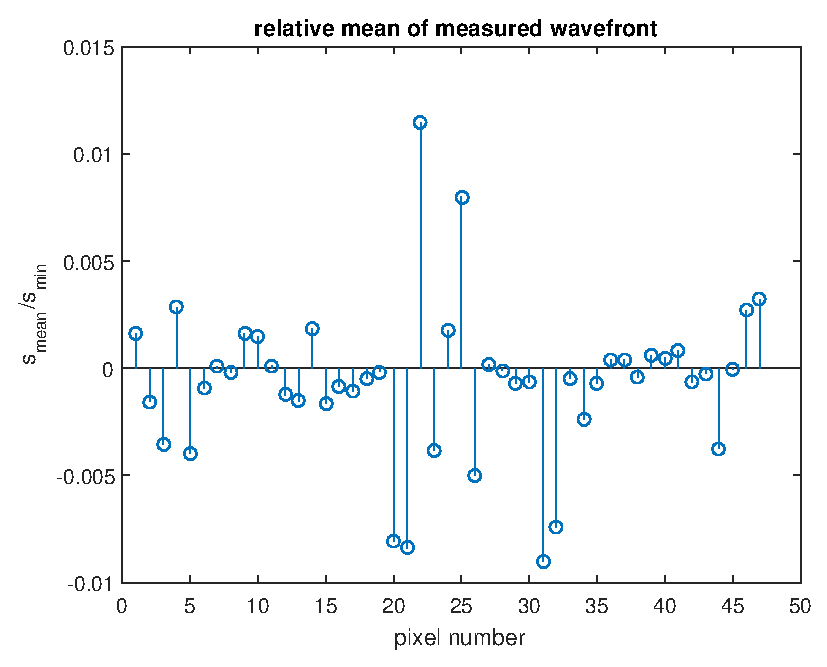
\includegraphics[width=0.8\textwidth]{figures/relative_mean.eps}
    \caption{Caption}
    \label{fig:rel_mean}
\end{figure}

\begin{figure}[H]
  \centering
  \includegraphics[width=0.8\textwidth]{figures/linear_trend.eps}
  \caption{test}
  \label{fig:linear_trend}
\end{figure}





%----------------------------------------------------------------------------------------
%  Comparison
%----------------------------------------------------------------------------------------
\chapter{\bf Comparison}

\bibliography{bibliography} 
\bibliographystyle{ieeetr}
\end{document}